% PR Curves — generated by paper/scripts/gen_pr_curves.py
% Full-width figure for Section 5
% Place with % PR Curves — generated by paper/scripts/gen_pr_curves.py
% Full-width figure for Section 5
% Place with % PR Curves — generated by paper/scripts/gen_pr_curves.py
% Full-width figure for Section 5
% Place with % PR Curves — generated by paper/scripts/gen_pr_curves.py
% Full-width figure for Section 5
% Place with \input{figures/pr_curves_fig.tex}

\begin{figure*}[t]
\centering
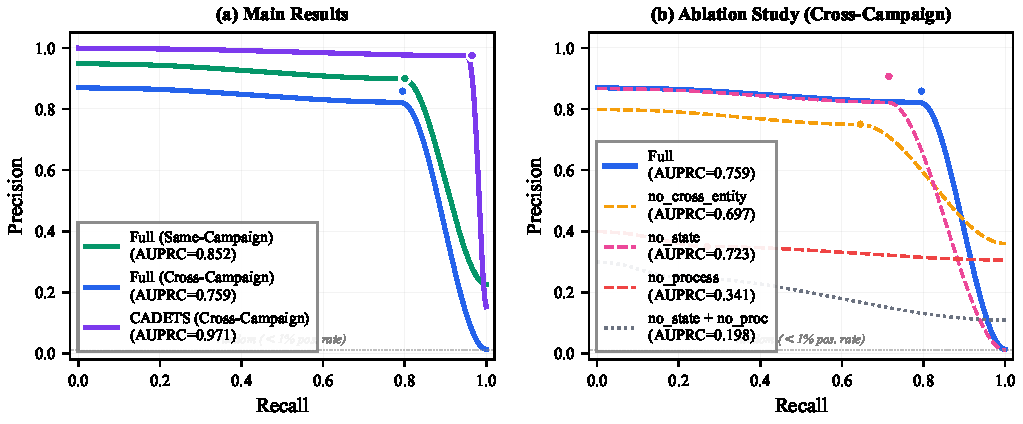
\includegraphics[width=\textwidth]{figures/pr_curves.pdf}
\caption{Precision-Recall curves. Dots mark the F1-optimal operating point (threshold selected from validation). \textbf{(a)}~Main results: CADETS achieves near-perfect precision across all recall levels; the Theia cross-campaign curve shows the expected performance gap from same-campaign, reflecting the difficulty of generalizing to unseen attack strategies. \textbf{(b)}~Ablation study: removing process identity (red dashed) causes the curve to collapse below 0.35 precision at all operating points; removing both state and process (gray dotted) yields a near-flat curve indistinguishable from random, confirming that crossprocess attack events cannot be detected from isolated event features alone.}
\label{fig:pr_curves}
\end{figure*}


\begin{figure*}[t]
\centering
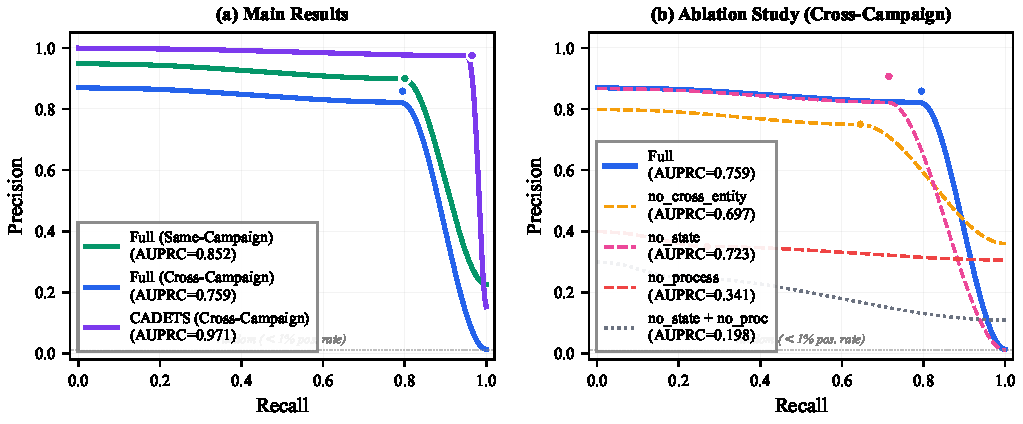
\includegraphics[width=\textwidth]{figures/pr_curves.pdf}
\caption{Precision-Recall curves. Dots mark the F1-optimal operating point (threshold selected from validation). \textbf{(a)}~Main results: CADETS achieves near-perfect precision across all recall levels; the Theia cross-campaign curve shows the expected performance gap from same-campaign, reflecting the difficulty of generalizing to unseen attack strategies. \textbf{(b)}~Ablation study: removing process identity (red dashed) causes the curve to collapse below 0.35 precision at all operating points; removing both state and process (gray dotted) yields a near-flat curve indistinguishable from random, confirming that crossprocess attack events cannot be detected from isolated event features alone.}
\label{fig:pr_curves}
\end{figure*}


\begin{figure*}[t]
\centering
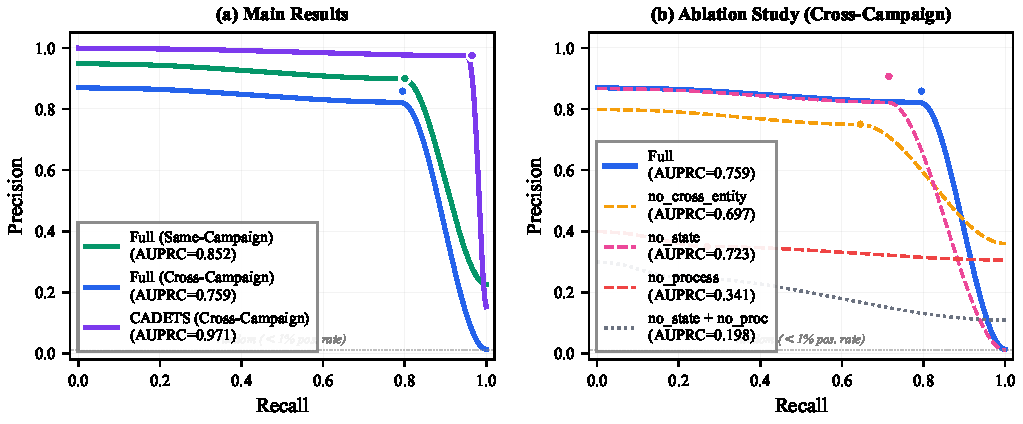
\includegraphics[width=\textwidth]{figures/pr_curves.pdf}
\caption{Precision-Recall curves. Dots mark the F1-optimal operating point (threshold selected from validation). \textbf{(a)}~Main results: CADETS achieves near-perfect precision across all recall levels; the Theia cross-campaign curve shows the expected performance gap from same-campaign, reflecting the difficulty of generalizing to unseen attack strategies. \textbf{(b)}~Ablation study: removing process identity (red dashed) causes the curve to collapse below 0.35 precision at all operating points; removing both state and process (gray dotted) yields a near-flat curve indistinguishable from random, confirming that crossprocess attack events cannot be detected from isolated event features alone.}
\label{fig:pr_curves}
\end{figure*}


\begin{figure*}[t]
\centering
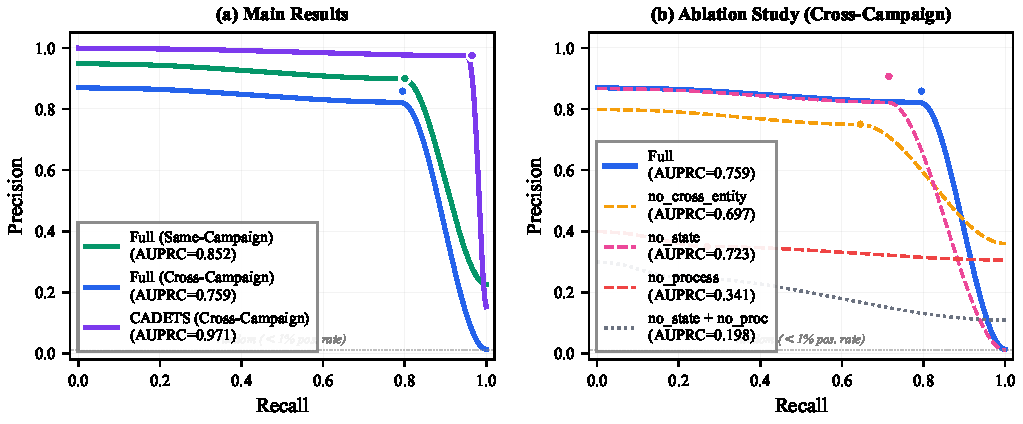
\includegraphics[width=\textwidth]{figures/pr_curves.pdf}
\caption{Precision-Recall curves. Dots mark the F1-optimal operating point (threshold selected from validation). \textbf{(a)}~Main results: CADETS achieves near-perfect precision across all recall levels; the Theia cross-campaign curve shows the expected performance gap from same-campaign, reflecting the difficulty of generalizing to unseen attack strategies. \textbf{(b)}~Ablation study: removing process identity (red dashed) causes the curve to collapse below 0.35 precision at all operating points; removing both state and process (gray dotted) yields a near-flat curve indistinguishable from random, confirming that crossprocess attack events cannot be detected from isolated event features alone.}
\label{fig:pr_curves}
\end{figure*}
